% This is based on "sig-alternate.tex" V1.9 April 2009
% This file should be compiled with V2.4 of "sig-alternate.cls" April 2009
%
% ----------------------------------------------------------------------------------------------------------------
%
% This .tex source is an example which *does* use
% the .bib file (from which the .bbl file % is produced).
% REMEMBER HOWEVER: After having produced the .bbl file,
% and prior to final submission, you *NEED* to 'insert'
% your .bbl file into your source .tex file so as to provide
% ONE 'self-contained' source file.
%
% Information on the sig-alternate class file and on the
% GECCO workshop paper format and submission can be found at these
% locations:
% http://www.acm.org/sigs/publications/proceedings-templates#aL2
% http://www.sheridanprinting.com/typedept/gecco3.htm
%
% ================= IF YOU HAVE QUESTIONS =======================
% Questions regarding the SIGS styles, SIGS policies and
% procedures, Conferences etc. should be sent to
% Adrienne Griscti (griscti@acm.org)
%
% Technical questions to bbob@lri.fr
% ===============================================================
%

\documentclass{sig-alternate}

\usepackage{graphicx}
\usepackage{rotating}
\pdfpagewidth=8.5in
\pdfpageheight=11in
\special{papersize=8.5in,11in}

    \renewcommand{\topfraction}{1}	% max fraction of floats at top
    \renewcommand{\bottomfraction}{1} % max fraction of floats at bottom
    %   Parameters for TEXT pages (not float pages):
    \setcounter{topnumber}{3}
    \setcounter{bottomnumber}{3}
    \setcounter{totalnumber}{3}     % 2 may work better
    \setcounter{dbltopnumber}{4}    % for 2-column pages
    \renewcommand{\dbltopfraction}{1}	% fit big float above 2-col. text
    \renewcommand{\textfraction}{0.0}	% allow minimal text w. figs
    %   Parameters for FLOAT pages (not text pages):
    \renewcommand{\floatpagefraction}{0.80}	% require fuller float pages
	% N.B.: floatpagefraction MUST be less than topfraction !!
    \renewcommand{\dblfloatpagefraction}{0.7}	% require fuller float pages

\newcommand{\DIM}{\ensuremath{\mathrm{DIM}}}
\newcommand{\ERT}{\ensuremath{\mathrm{ERT}}}
\newcommand{\FEvals}{\ensuremath{\mathrm{FEvals}}}
\newcommand{\nruns}{\ensuremath{\mathrm{Nruns}}}
\newcommand{\Dfb}{\ensuremath{\Delta f_{\mathrm{best}}}}
\newcommand{\Df}{\ensuremath{\Delta f}}
\newcommand{\nbFEs}{\ensuremath{\mathrm{\#FEs}}}
\newcommand{\fopt}{\ensuremath{f_\mathrm{opt}}}
\newcommand{\ftarget}{\ensuremath{f_\mathrm{t}}}
\newcommand{\CrE}{\ensuremath{\mathrm{CrE}}}

\newcommand{\bbobdatapath}{ppdata/}
\graphicspath{{\bbobdatapath}}

\begin{document}
%
% --- Author Metadata here ---
\conferenceinfo{GECCO'10,} {July 7--11, 2010, Portland, Oregon, USA.}
\CopyrightYear{2010}
\crdata{978-1-4503-0073-5/10/07}
\clubpenalty=10000
\widowpenalty = 10000
% --- End of Author Metadata ---

\title{Black-Box Optimization Benchmarking Template for Noiseless Function
Testbed
% \titlenote{If needed}
}
\subtitle{Draft version
\titlenote{Submission deadline: March 25th.}}
%Camera-ready paper due April 13th.}}

%
% You need the command \numberofauthors to handle the 'placement
% and alignment' of the authors beneath the title.
%
% For aesthetic reasons, we recommend 'three authors at a time'
% i.e. three 'name/affiliation blocks' be placed beneath the title.
%
% NOTE: You are NOT restricted in how many 'rows' of
% "name/affiliations" may appear. We just ask that you restrict
% the number of 'columns' to three.
%
% Because of the available 'opening page real-estate'
% we ask you to refrain from putting more than six authors
% (two rows with three columns) beneath the article title.
% More than six makes the first-page appear very cluttered indeed.
%
% Use the \alignauthor commands to handle the names
% and affiliations for an 'aesthetic maximum' of six authors.
% Add names, affiliations, addresses for
% the seventh etc. author(s) as the argument for the
% \additionalauthors command.
% These 'additional authors' will be output/set for you
% without further effort on your part as the last section in
% the body of your article BEFORE References or any Appendices.

\numberofauthors{1} %  in this sample file, there are a *total*
% of EIGHT authors. SIX appear on the 'first-page' (for formatting
% reasons) and the remaining two appear in the \additionalauthors section.
%
\author{
% You can go ahead and credit any number of authors here,
% e.g. one 'row of three' or two rows (consisting of one row of three
% and a second row of one, two or three).
%
% The command \alignauthor (no curly braces needed) should
% precede each author name, affiliation/snail-mail address and
% e-mail address. Additionally, tag each line of
% affiliation/address with \affaddr, and tag the
% e-mail address with \email.
%
% 1st. author
\alignauthor
Forename Name\\ %\titlenote{Dr.~Trovato insisted his name be first.}\\
%       \affaddr{Institute for Clarity in Documentation}\\
%       \affaddr{1932 Wallamaloo Lane}\\
%       \affaddr{Wallamaloo, New Zealand}\\
%       \email{trovato@corporation.com}
%% 2nd. author
%\alignauthor
%G.K.M. Tobin\titlenote{The secretary disavows
%any knowledge of this author's actions.}\\
%       \affaddr{Institute for Clarity in Documentation}\\
%       \affaddr{P.O. Box 1212}\\
%       \affaddr{Dublin, Ohio 43017-6221}\\
%       \email{webmaster@marysville-ohio.com}
%% 3rd. author
%\alignauthor Lars Th{\o}rv{\"a}ld\titlenote{This author is the
%one who did all the really hard work.}\\
%       \affaddr{The Th{\o}rv{\"a}ld Group}\\
%       \affaddr{1 Th{\o}rv{\"a}ld Circle}\\
%       \affaddr{Hekla, Iceland}\\
%       \email{larst@affiliation.org}
%\and  % use '\and' if you need 'another row' of author names
%% 4th. author
%\alignauthor Lawrence P. Leipuner\\
%       \affaddr{Brookhaven Laboratories}\\
%       \affaddr{Brookhaven National Lab}\\
%       \affaddr{P.O. Box 5000}\\
%       \email{lleipuner@researchlabs.org}
%% 5th. author
%\alignauthor Sean Fogarty\\
%       \affaddr{NASA Ames Research Center}\\
%       \affaddr{Moffett Field}\\
%       \affaddr{California 94035}\\
%       \email{fogartys@amesres.org}
%% 6th. author
%\alignauthor Charles Palmer\\
%       \affaddr{Palmer Research Laboratories}\\
%       \affaddr{8600 Datapoint Drive}\\
%       \affaddr{San Antonio, Texas 78229}\\
%       \email{cpalmer@prl.com}
} % author
%% There's nothing stopping you putting the seventh, eighth, etc.
%% author on the opening page (as the 'third row') but we ask,
%% for aesthetic reasons that you place these 'additional authors'
%% in the \additional authors block, viz.
%\additionalauthors{Additional authors: John Smith (The Th{\o}rv{\"a}ld Group,
%email: {\texttt{jsmith@affiliation.org}}) and Julius P.~Kumquat
%(The Kumquat Consortium, email: {\texttt{jpkumquat@consortium.net}}).}
%\date{30 July 1999}
%% Just remember to make sure that the TOTAL number of authors
%% is the number that will appear on the first page PLUS the
%% number that will appear in the \additionalauthors section.

\maketitle
\begin{abstract}
\end{abstract}

% Add any ACM category that you feel is needed
\category{G.1.6}{Numerical Analysis}{Optimization}[global optimization,
unconstrained optimization]
\category{F.2.1}{Analysis of Algorithms and Problem Complexity}{Numerical Algorithms and Problems}

% Complete with anything that is needed
\terms{Algorithms}

% Complete with anything that is needed
\keywords{Benchmarking, Black-box optimization}

% \section{Introduction}
%
% \section{Algorithm Presentation}
%
% \section{Experimental Procedure}
%
%%%%%%%%%%%%%%%%%%%%%%%%%%%%%%%%%%%%%%%%%%%%%%%%%%%%%%%%%%%%%%%%%%%%%%%%%%%%%%%
\section{Results}
%%%%%%%%%%%%%%%%%%%%%%%%%%%%%%%%%%%%%%%%%%%%%%%%%%%%%%%%%%%%%%%%%%%%%%%%%%%%%%%

Results from experiments according to \cite{hansen2010exp} on the benchmark
functions given in \cite{wp200901_2010,hansen2010fun} are presented in
Figures~\ref{fig:ERTgraphs}, \ref{fig:RLDs} and \ref{fig:ERTlogloss} and in
Tables~\ref{tab:ERTs} and \ref{tab:ERTloss}.
%%%%%%%%%%%%%%%%%%%%%%%%%%%%%%%%%%%%%%%%%%%%%%%%%%%%%%%%%%%%%%%%%%%%%%%%%%%%%%%
\begin{figure*}
\begin{tabular}{l@{\hspace*{-0.025\textwidth}}l@{\hspace*{-0.025\textwidth}}l@{\hspace*{-0.025\textwidth}}l}
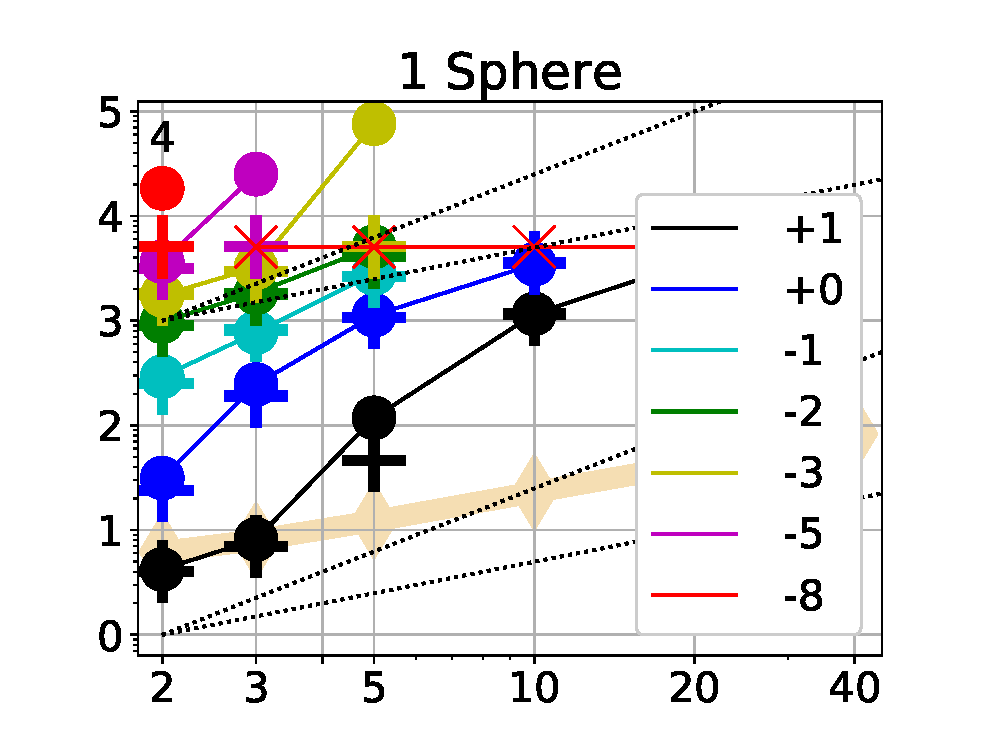
\includegraphics[width=0.268\textwidth]{ppdata_f1}&
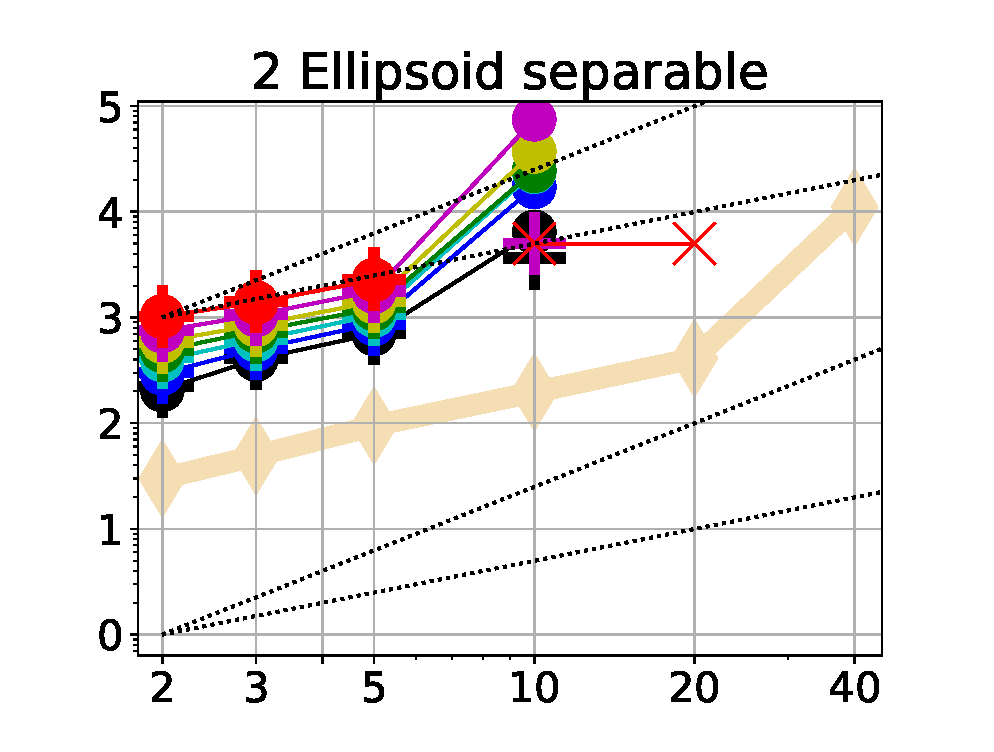
\includegraphics[width=0.268\textwidth]{ppdata_f2}&
\includegraphics[width=0.268\textwidth]{ppdata_f3}&
\includegraphics[width=0.268\textwidth]{ppdata_f4}\\[-2.2ex]
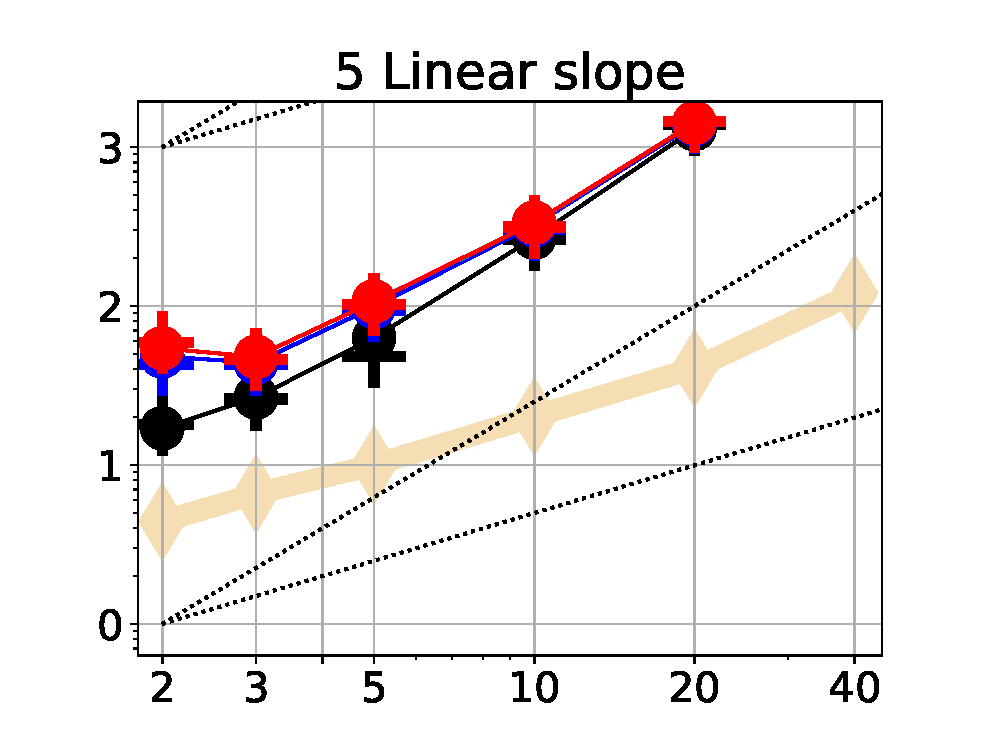
\includegraphics[width=0.268\textwidth]{ppdata_f5}&
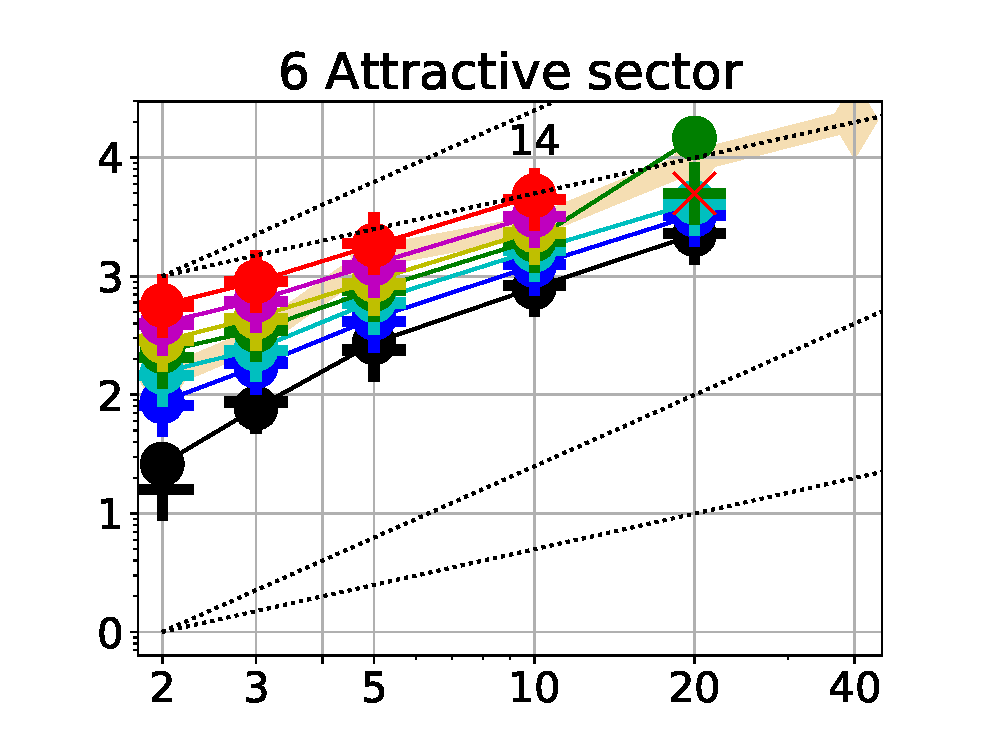
\includegraphics[width=0.268\textwidth]{ppdata_f6}&
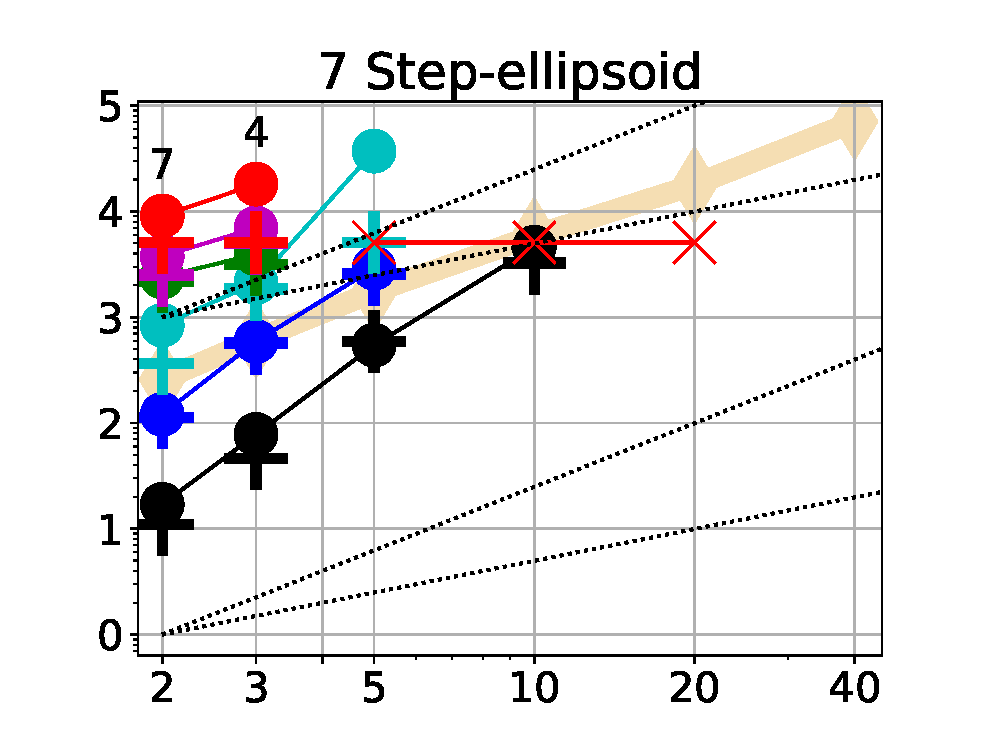
\includegraphics[width=0.268\textwidth]{ppdata_f7}&
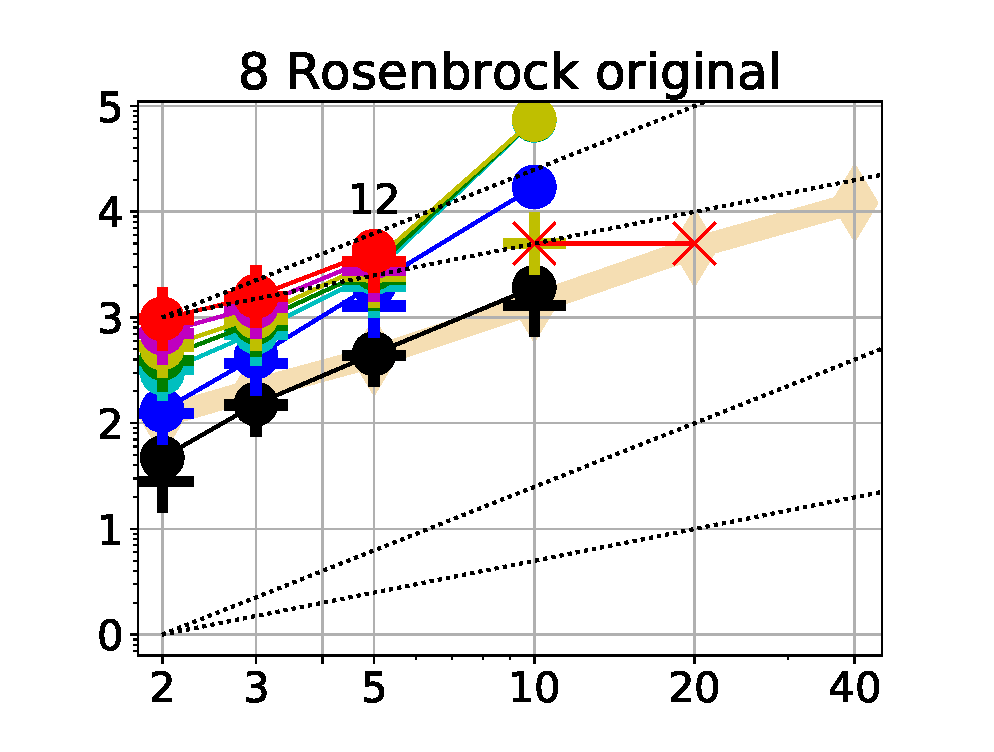
\includegraphics[width=0.268\textwidth]{ppdata_f8}\\[-2.2ex]
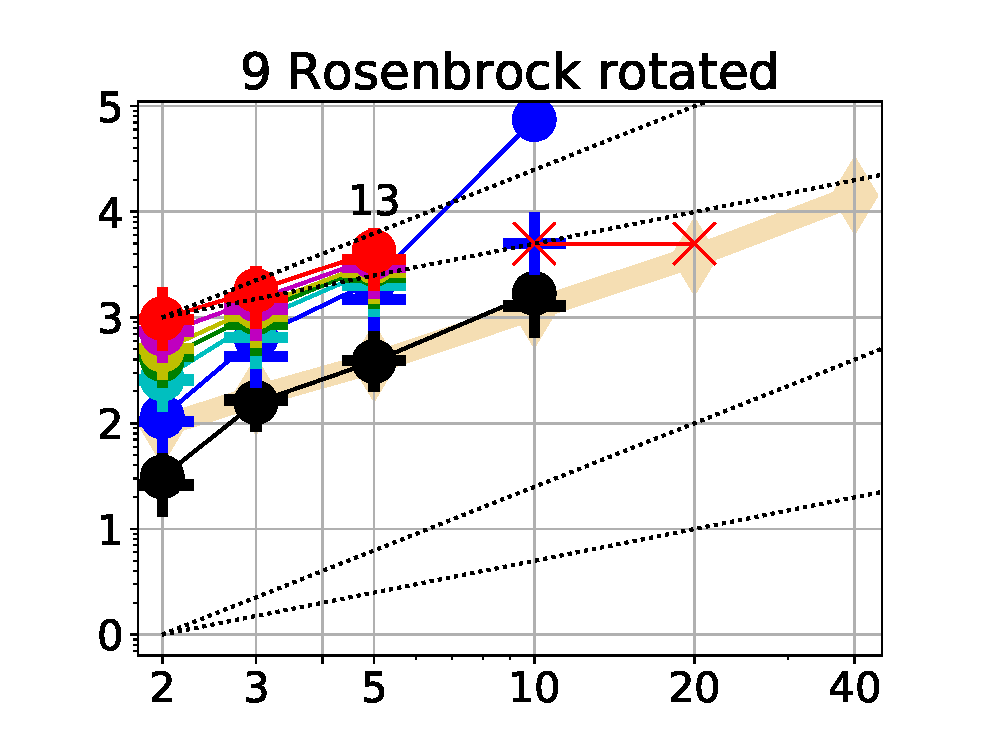
\includegraphics[width=0.268\textwidth]{ppdata_f9}&
\includegraphics[width=0.268\textwidth]{ppdata_f10}&
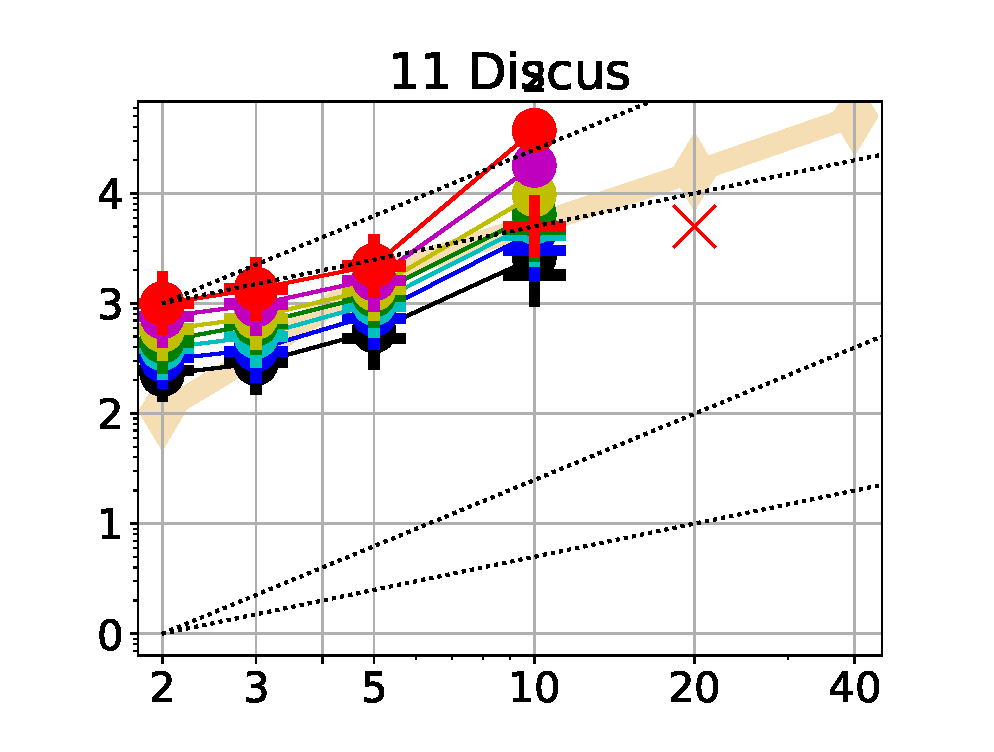
\includegraphics[width=0.268\textwidth]{ppdata_f11}&
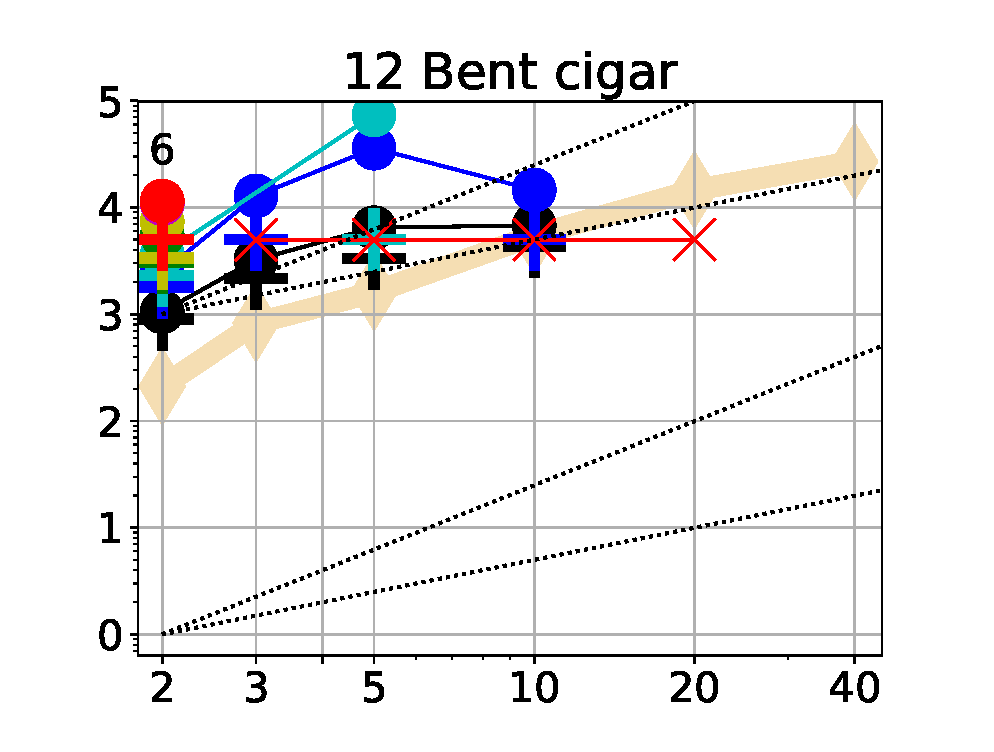
\includegraphics[width=0.268\textwidth]{ppdata_f12}\\[-2.2ex]
\includegraphics[width=0.268\textwidth]{ppdata_f13}&
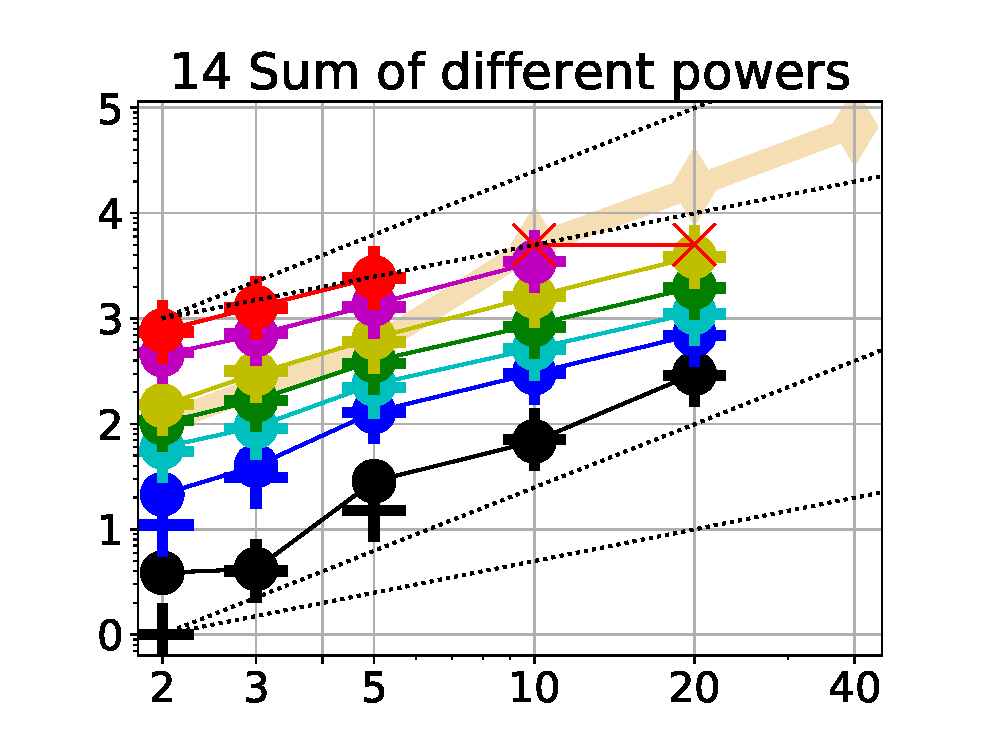
\includegraphics[width=0.268\textwidth]{ppdata_f14}&
\includegraphics[width=0.268\textwidth]{ppdata_f15}&
\includegraphics[width=0.268\textwidth]{ppdata_f16}\\[-2.2ex]
\includegraphics[width=0.268\textwidth]{ppdata_f17}&
\includegraphics[width=0.268\textwidth]{ppdata_f18}&
\includegraphics[width=0.268\textwidth]{ppdata_f19}&
\includegraphics[width=0.268\textwidth]{ppdata_f20}\\[-2.2ex]
\includegraphics[width=0.268\textwidth]{ppdata_f21}&
\includegraphics[width=0.268\textwidth]{ppdata_f22}&
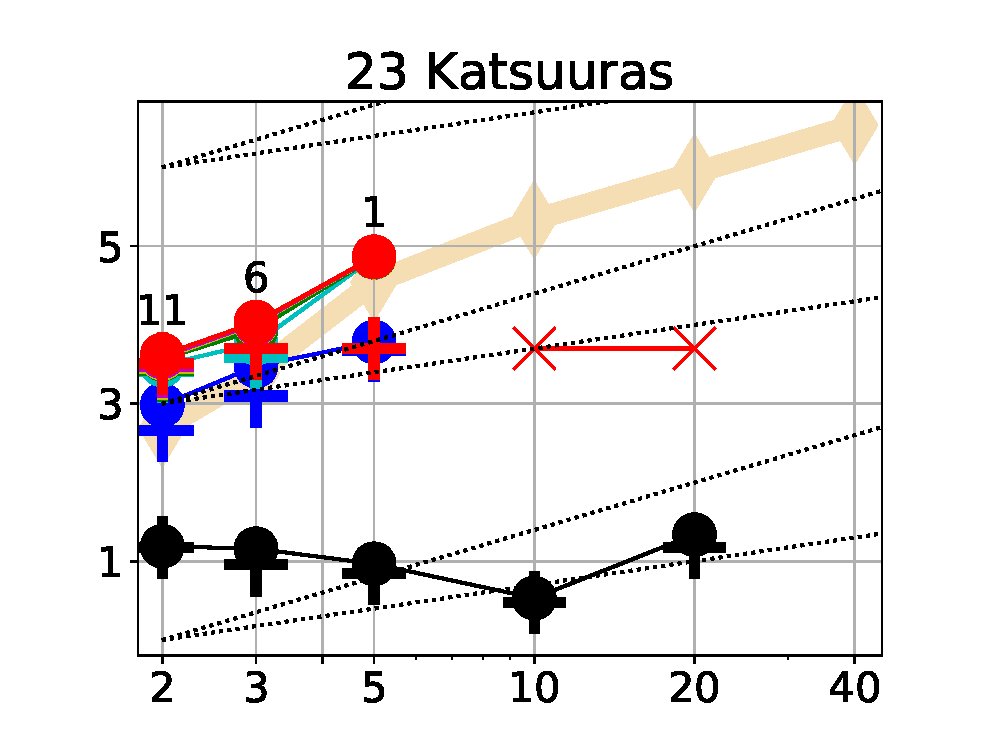
\includegraphics[width=0.268\textwidth]{ppdata_f23}&
\includegraphics[width=0.268\textwidth]{ppdata_f24}
\end{tabular}
\vspace{-3ex}
 \caption{\label{fig:ERTgraphs}Expected Running Time (\ERT,
 {\Large$\bullet$}) to reach $\fopt+\Df$ and median number of
 $f$-evaluations from successful trials ($+$), for 
% $\Df = 10, 1, 10^{-1}, 10^{-2}, 10^{-3}, 10^{-5}, 10^{-8}$ 
$\Df = 10^{\{+1, 0, -1, -2, -3, -5, -8\}}$ 
 (the exponent is given in the legend of 
%
$f_1$ and $f_{24}$) 
%
 versus dimension in log-log presentation. For each function 
 and dimension, $\ERT(\Df)$ equals to $\nbFEs(\Df)$
 divided by the number of successful trials, where a trial is
 successful if $\fopt+\Df$ was surpassed. The
 $\nbFEs(\Df)$ are the total number (sum) of $f$-evaluations while
 $\fopt+\Df$ was not surpassed in the trial, from all  
 (successful and unsuccessful) trials, and \fopt\ is the optimal
 function value. Crosses ($\times$) indicate the total number of
 $f$-evaluations, $\nbFEs(-\infty)$, divided by the number of trials.
 Numbers above ERT-symbols indicate the number of successful trials.
 Y-axis annotations are decimal logarithms. The thick light
 line with diamonds shows the single best results from BBOB-2009 for 
 $\Df=10^{-8}$. Additional grid lines show linear and quadratic scaling. }
\end{figure*}

%%%%%%%%%%%%%%%%%%%%%%%%%%%%%%%%%%%%%%%%%%%%%%%%%%%%%%%%%%%%%%%%%%%%%%%%%%%%%%%
%%%%%%%%%%%%%%%%%%%%%%%%%%%%%%%%%%%%%%%%%%%%%%%%%%%%%%%%%%%%%%%%%%%%%%%%%%%%%%%
 \newcommand{\tablecaption}{Shown are, for a given target difference
 to the optimal function value \Df: the number of successful trials
 (\textbf{$\#$}); the expected running time to surpass $\fopt+\Df$
 (\ERT, see Figure~\ref{fig:ERTgraphs}); the \textbf{10\%}-tile and
 \textbf{90\%}-tile of the bootstrap distribution of \ERT; the average
 number of function evaluations in successful trials or, if none was
 successful, as last entry the median number of function evaluations
 to reach the best function value ($\text{RT}_\text{succ}$).  If
 $\fopt+\Df$ was never reached, figures in \textit{italics} denote the
 best achieved \Df-value of the median trial and the 10\% and
 90\%-tile trial.  Furthermore, N denotes the number of trials, and
 mFE denotes the maximum of number of function evaluations executed in
 one trial. See Figure~\ref{fig:ERTgraphs} for the names of
 functions. }
\begin{table*}
\centering
\input{\bbobdatapath ppdata_f1}
\input{\bbobdatapath ppdata_f2}
\input{\bbobdatapath ppdata_f3}
\input{\bbobdatapath ppdata_f4}
\input{\bbobdatapath ppdata_f5}
\input{\bbobdatapath ppdata_f6}
\input{\bbobdatapath ppdata_f7}
\input{\bbobdatapath ppdata_f8}
\input{\bbobdatapath ppdata_f9}
\input{\bbobdatapath ppdata_f10}
\input{\bbobdatapath ppdata_f11}
\input{\bbobdatapath ppdata_f12}
% %
%  \caption{\tablecaption
%  }
% \end{table*}
% %%%%%%%%%%%%%%%%%%%%%%%%%%%%%%%%%%%%%%%%%%%%%%%%%%%%%%%%%%%%%%%%%%%%%%%%%%%%%%%
% %%%%%%%%%%%%%%%%%%%%%%%%%%%%%%%%%%%%%%%%%%%%%%%%%%%%%%%%%%%%%%%%%%%%%%%%%%%%%%%
% \begin{table*}
% \centering
\input{\bbobdatapath ppdata_f13}
\input{\bbobdatapath ppdata_f14}
\input{\bbobdatapath ppdata_f15}
\input{\bbobdatapath ppdata_f16}
\input{\bbobdatapath ppdata_f17}
\input{\bbobdatapath ppdata_f18}
\input{\bbobdatapath ppdata_f19}
\input{\bbobdatapath ppdata_f20}
\input{\bbobdatapath ppdata_f21}
\input{\bbobdatapath ppdata_f22}
\input{\bbobdatapath ppdata_f23}
\input{\bbobdatapath ppdata_f24}\\
\caption[Table of ERTs]{\label{tab:ERTs}\tablecaption
}
\end{table*}

%%%%%%%%%%%%%%%%%%%%%%%%%%%%%%%%%%%%%%%%%%%%%%%%%%%%%%%%%%%%%%%%%%%%%%%%%%%%%%%
%%%%%%%%%%%%%%%%%%%%%%%%%%%%%%%%%%%%%%%%%%%%%%%%%%%%%%%%%%%%%%%%%%%%%%%%%%%%%%%
\newcommand{\rot}[2][2.5]{
  \hspace*{-3.5\baselineskip}%
  \begin{rotate}{90}\hspace{#1em}#2
  \end{rotate}}
\begin{figure*}
\begin{tabular}{l@{\hspace*{-0.025\textwidth}}l@{\hspace*{-0.00\textwidth}}|l@{\hspace*{-0.025\textwidth}}l}
\multicolumn{2}{c}{$D=5$} & \multicolumn{2}{c}{$D=20$}\\[-0.5ex]
\rot{all functions}
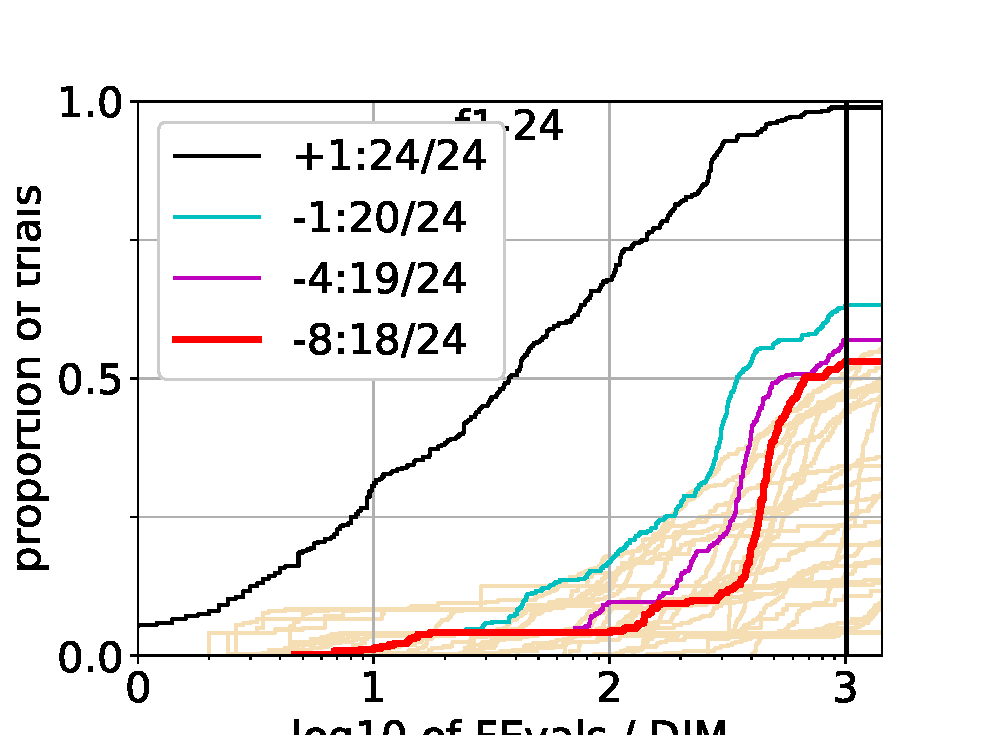
\includegraphics[width=0.268\textwidth,trim=0 0 0 13mm, clip]{pprldistr_dim05noiselessall} &
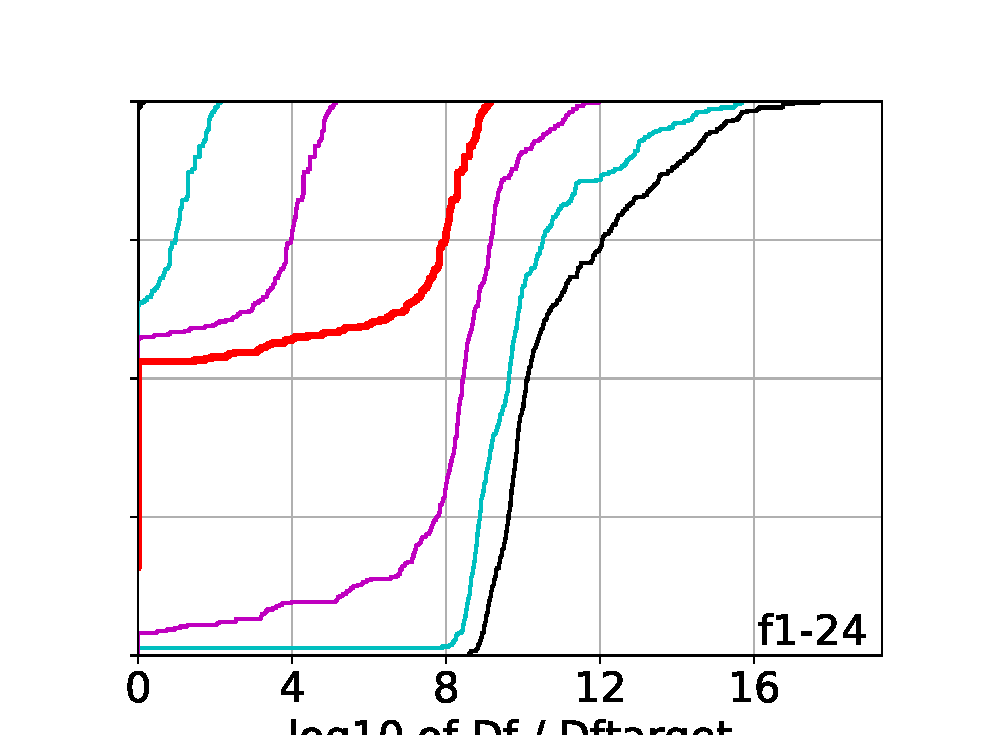
\includegraphics[width=0.2362\textwidth,trim=2.40cm 0 0 13mm, clip]{ppfvdistr_dim05noiselessall} &
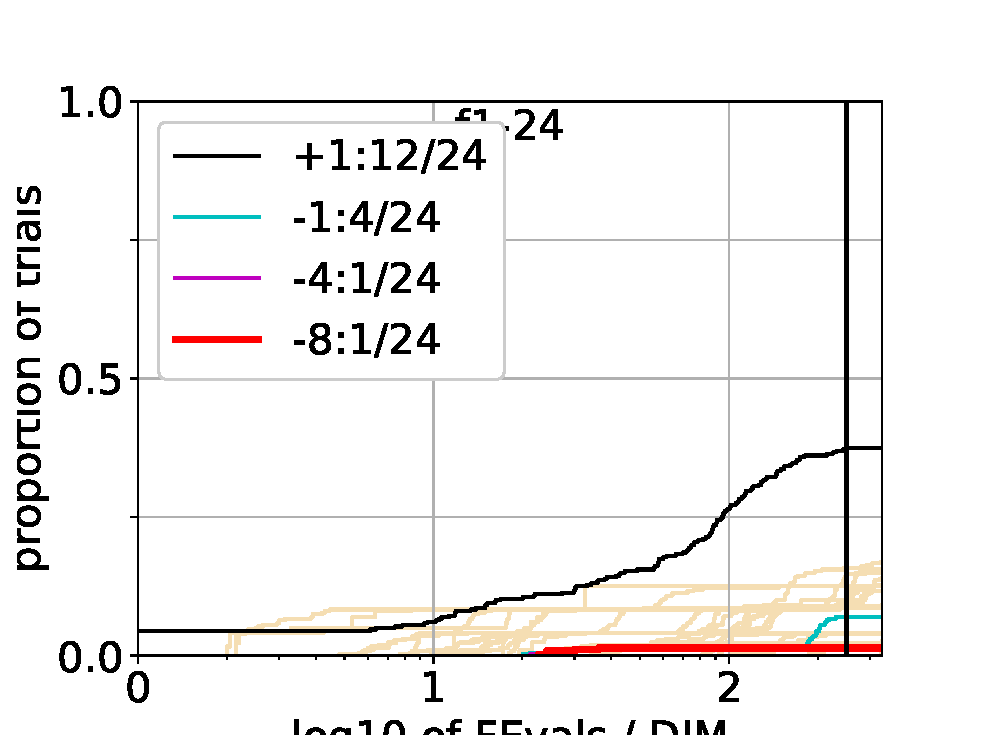
\includegraphics[width=0.268\textwidth,trim=0 0 0 13mm, clip]{pprldistr_dim20noiselessall} &
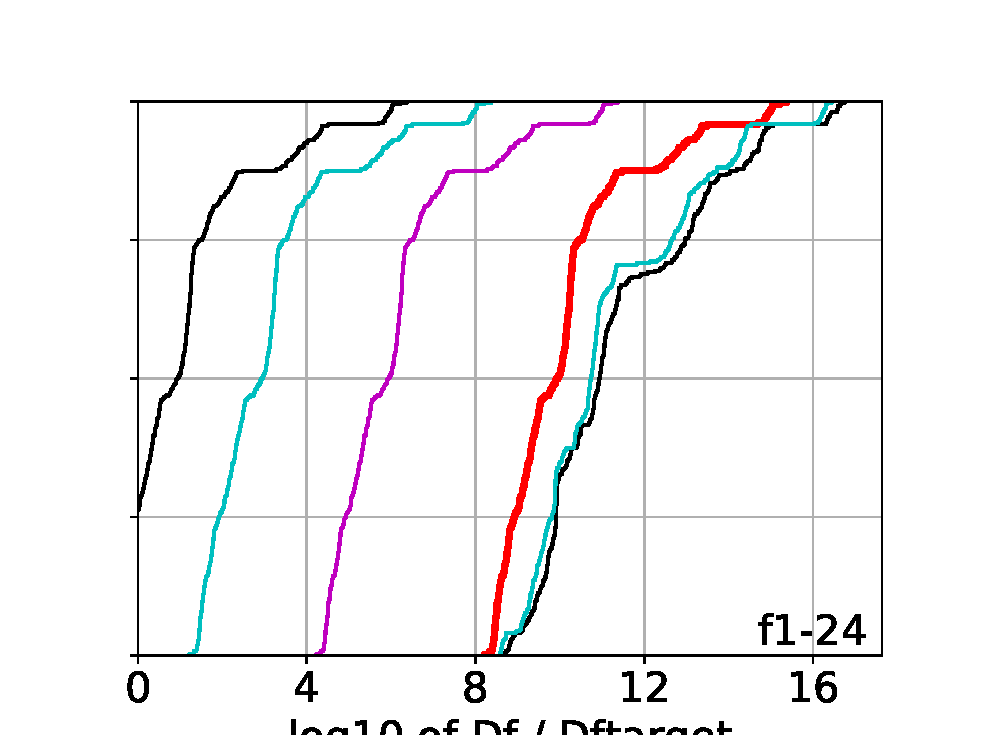
\includegraphics[width=0.2362\textwidth,trim=2.40cm 0 0 13mm, clip]{ppfvdistr_dim20noiselessall}
\\[-2ex]
\rot{separable fcts}
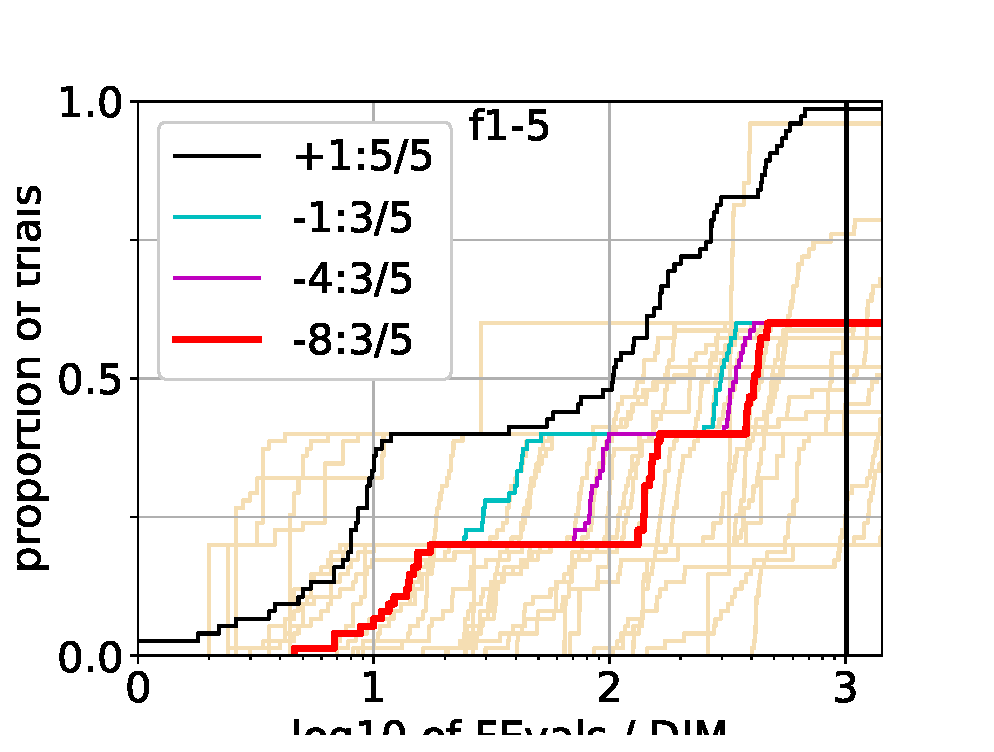
\includegraphics[width=0.268\textwidth,trim=0 0 0 13mm, clip]{pprldistr_dim05separ} &
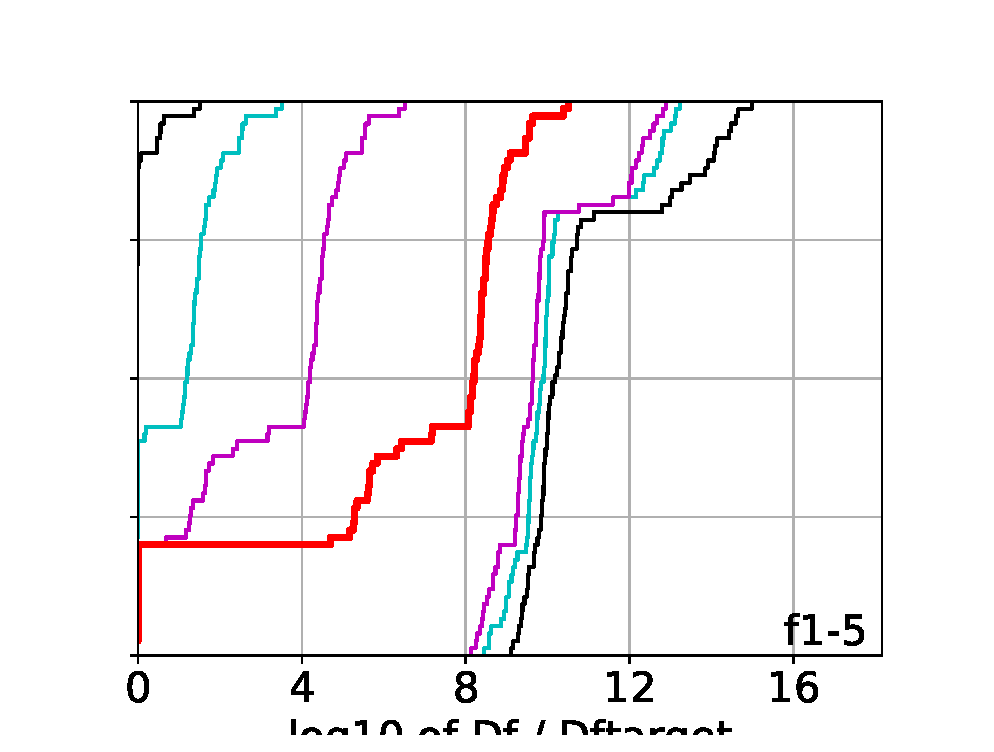
\includegraphics[width=0.2362\textwidth,trim=2.40cm 0 0 13mm, clip]{ppfvdistr_dim05separ} &
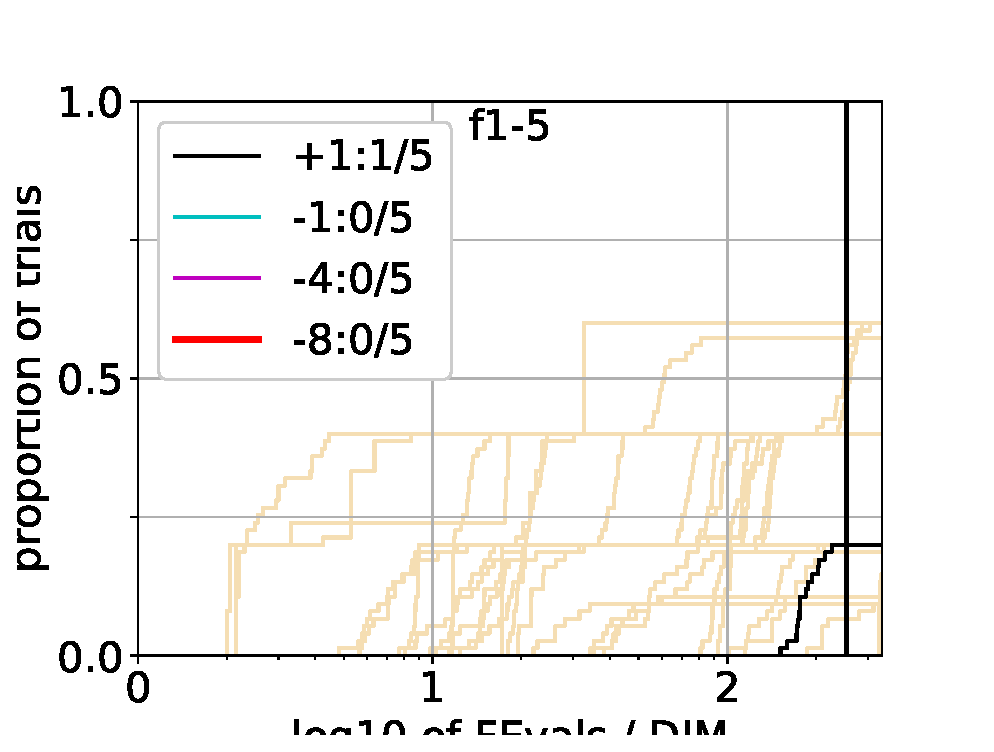
\includegraphics[width=0.268\textwidth,trim=0 0 0 13mm, clip]{pprldistr_dim20separ} &
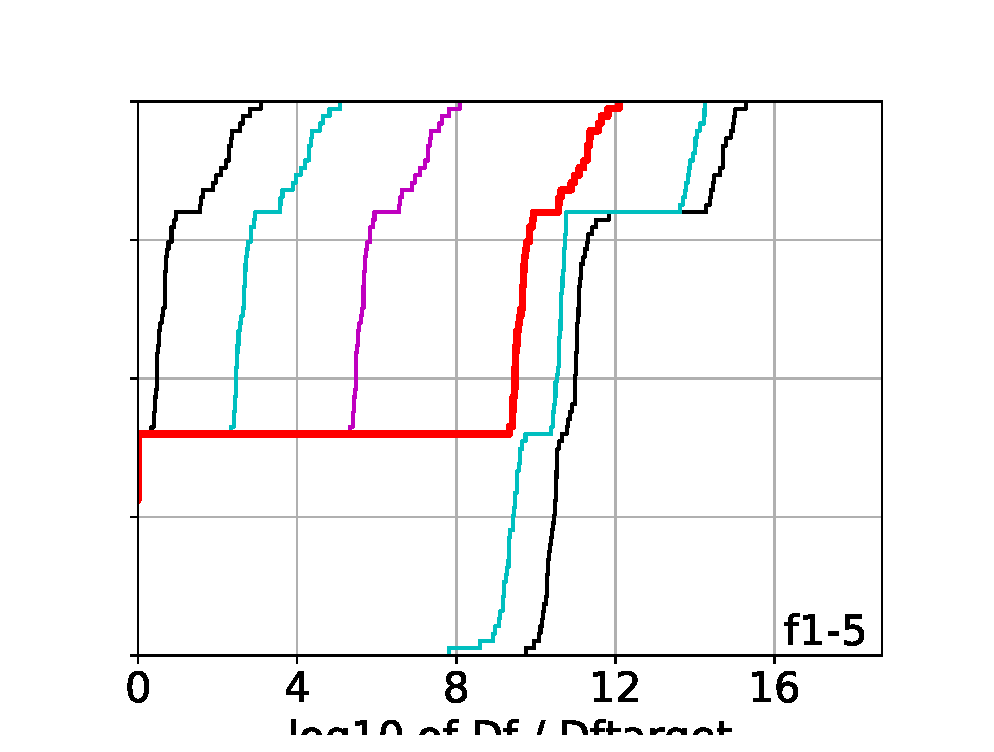
\includegraphics[width=0.2362\textwidth,trim=2.40cm 0 0 13mm, clip]{ppfvdistr_dim20separ} \\[-2ex]
\rot[1]{misc.\ moderate fcts}
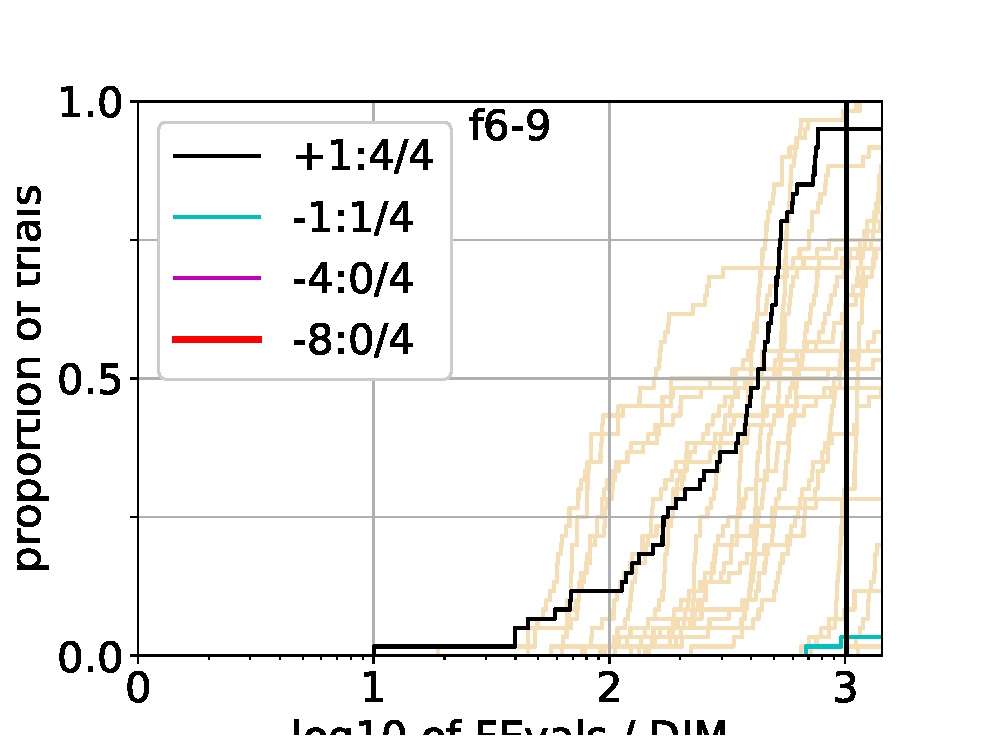
\includegraphics[width=0.268\textwidth,trim=0 0 0 13mm, clip]{pprldistr_dim05lcond} &
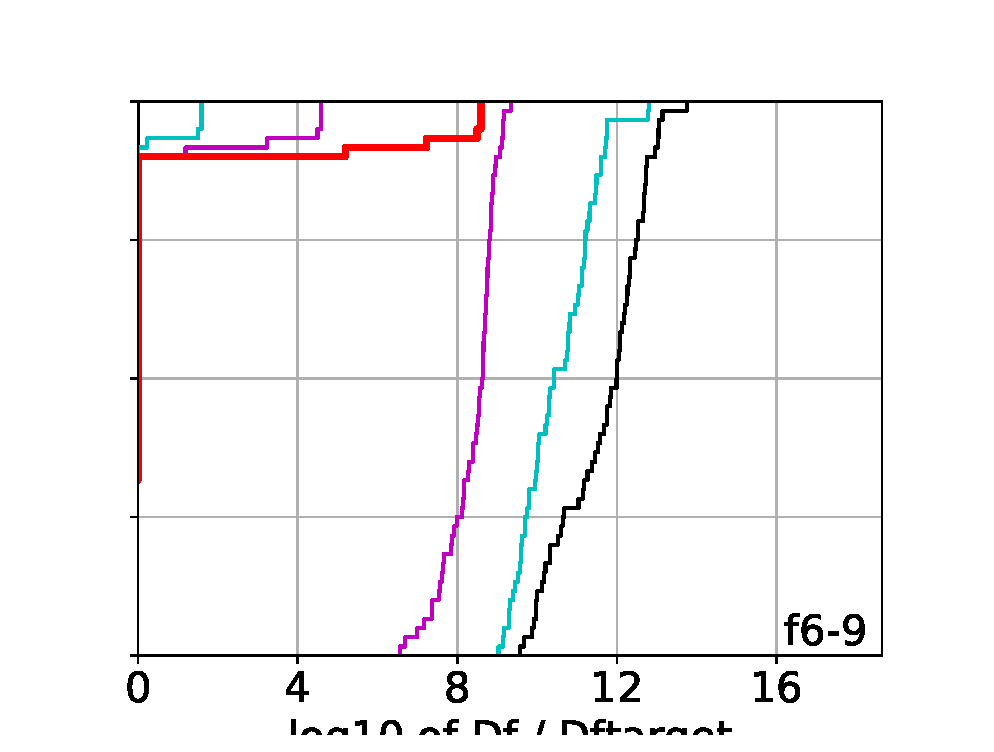
\includegraphics[width=0.23628\textwidth,trim=2.40cm 0 0 13mm, clip]{ppfvdistr_dim05lcond} &
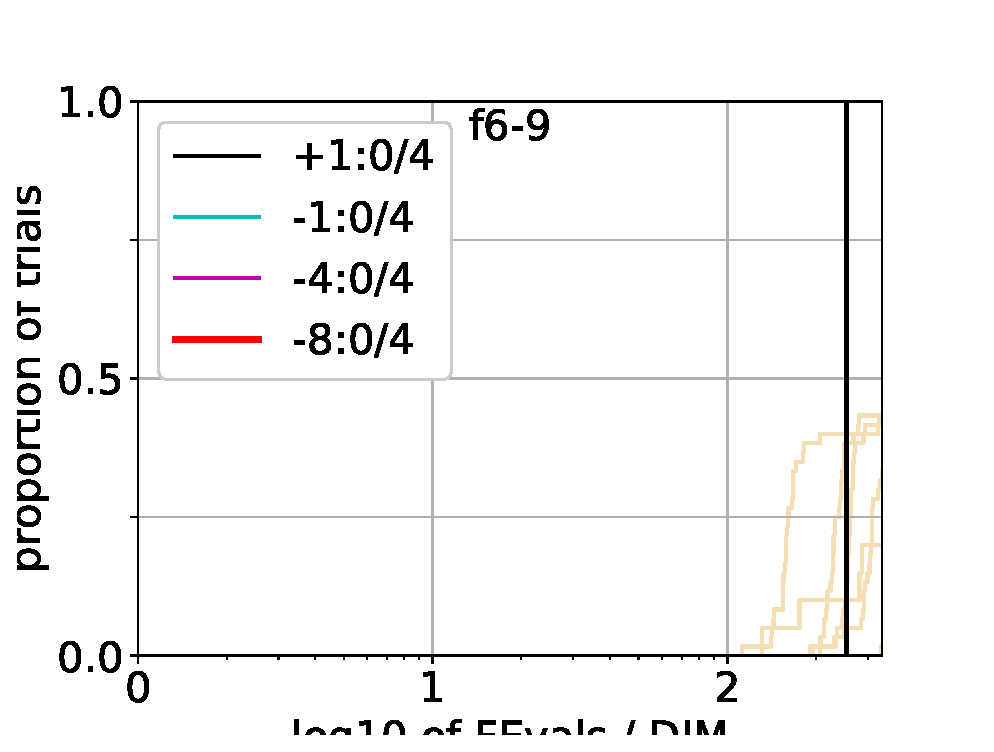
\includegraphics[width=0.268\textwidth,trim=0 0 0 13mm, clip]{pprldistr_dim20lcond} &
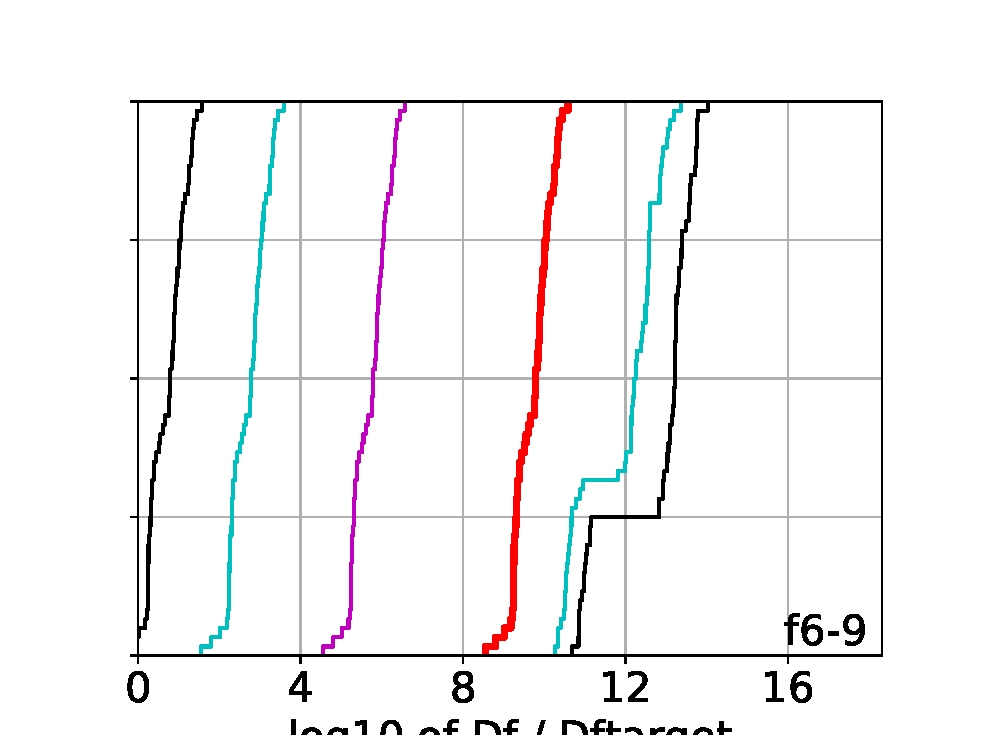
\includegraphics[width=0.2362\textwidth,trim=2.40cm 0 0 13mm, clip]{ppfvdistr_dim20lcond} \\[-2ex]
\rot[1.3]{ill-conditioned fcts}
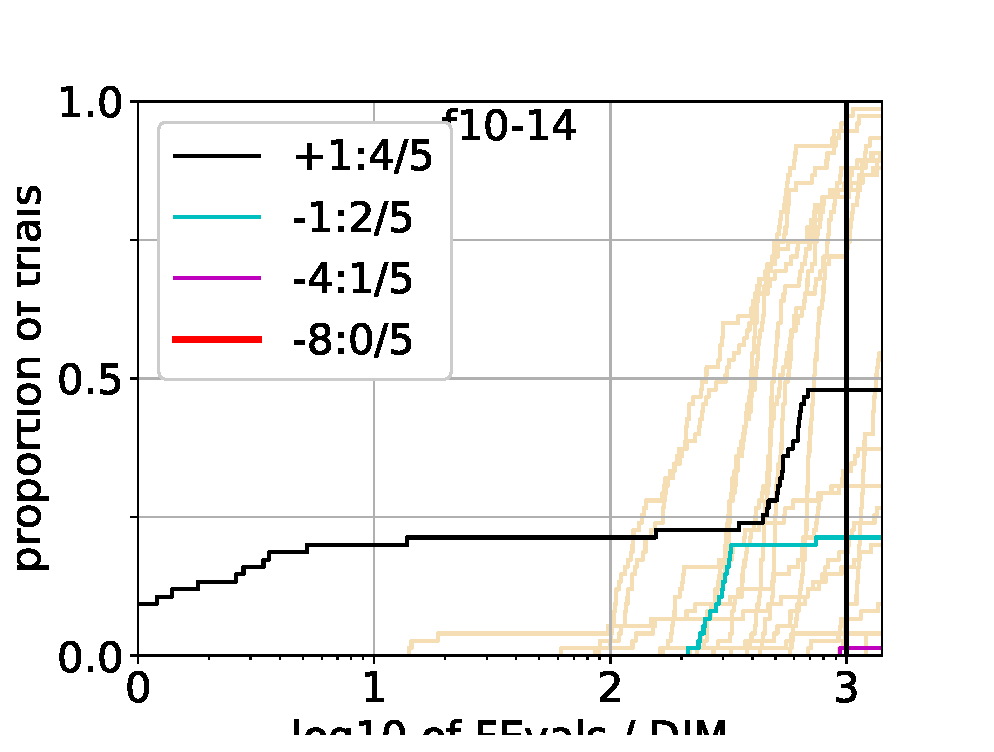
\includegraphics[width=0.268\textwidth,trim=0 0 0 13mm, clip]{pprldistr_dim05hcond} &
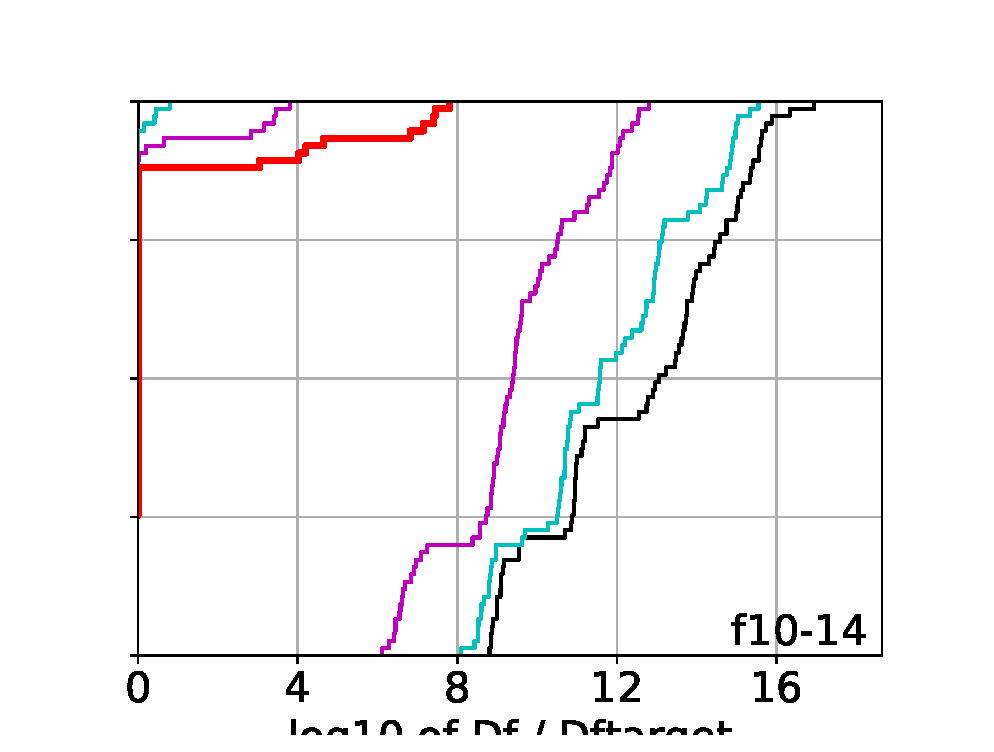
\includegraphics[width=0.2362\textwidth,trim=2.40cm 0 0 13mm, clip]{ppfvdistr_dim05hcond} &
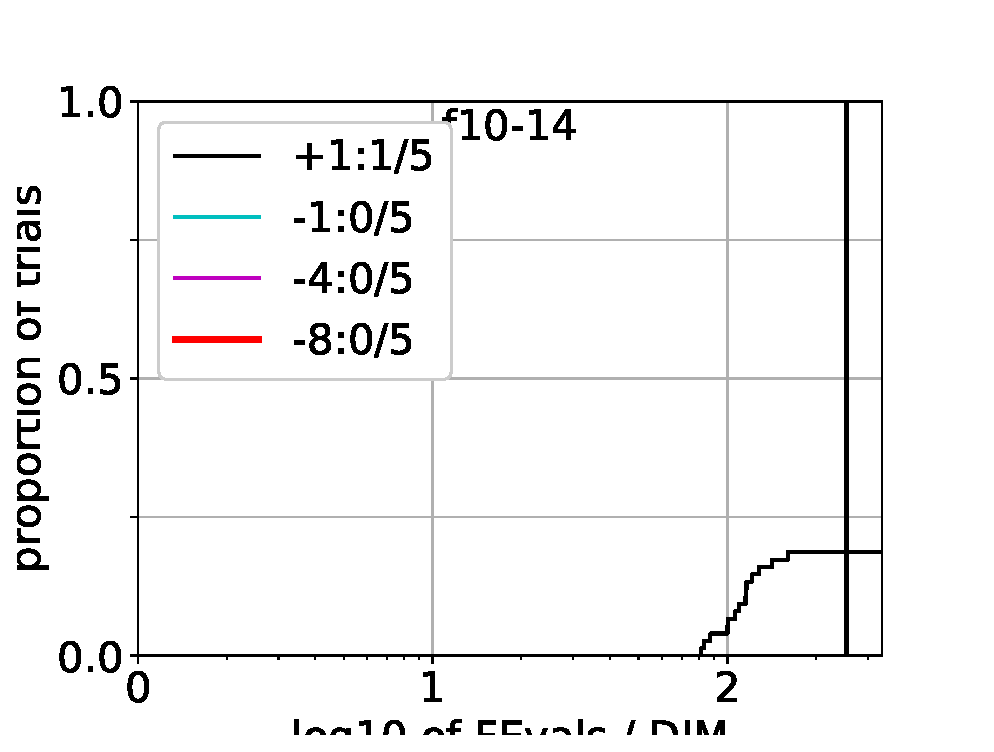
\includegraphics[width=0.268\textwidth,trim=0 0 0 13mm, clip]{pprldistr_dim20hcond} &
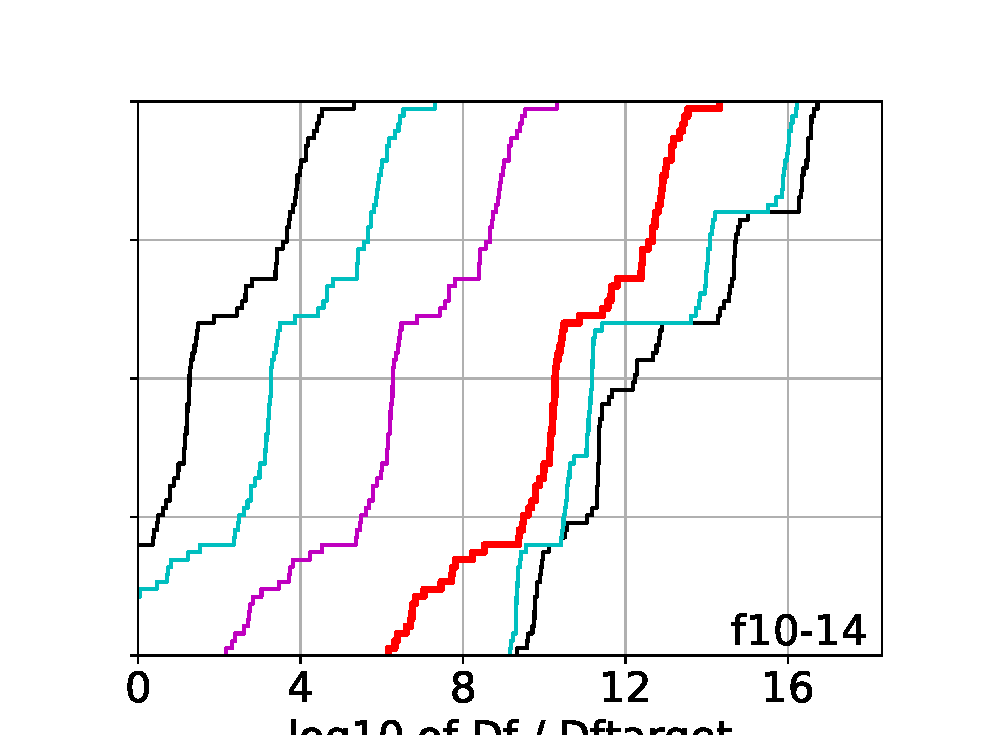
\includegraphics[width=0.2362\textwidth,trim=2.40cm 0 0 13mm, clip]{ppfvdistr_dim20hcond} \\[-2ex]
\rot[1.6]{multi-modal fcts}
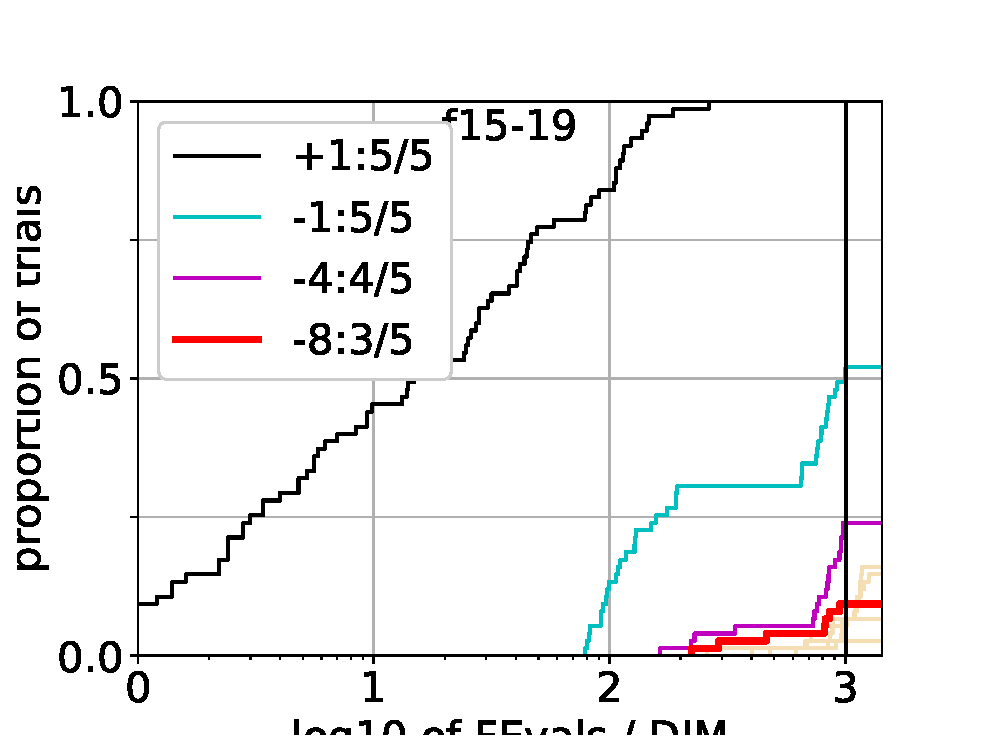
\includegraphics[width=0.268\textwidth,trim=0 0 0 13mm, clip]{pprldistr_dim05multi} &
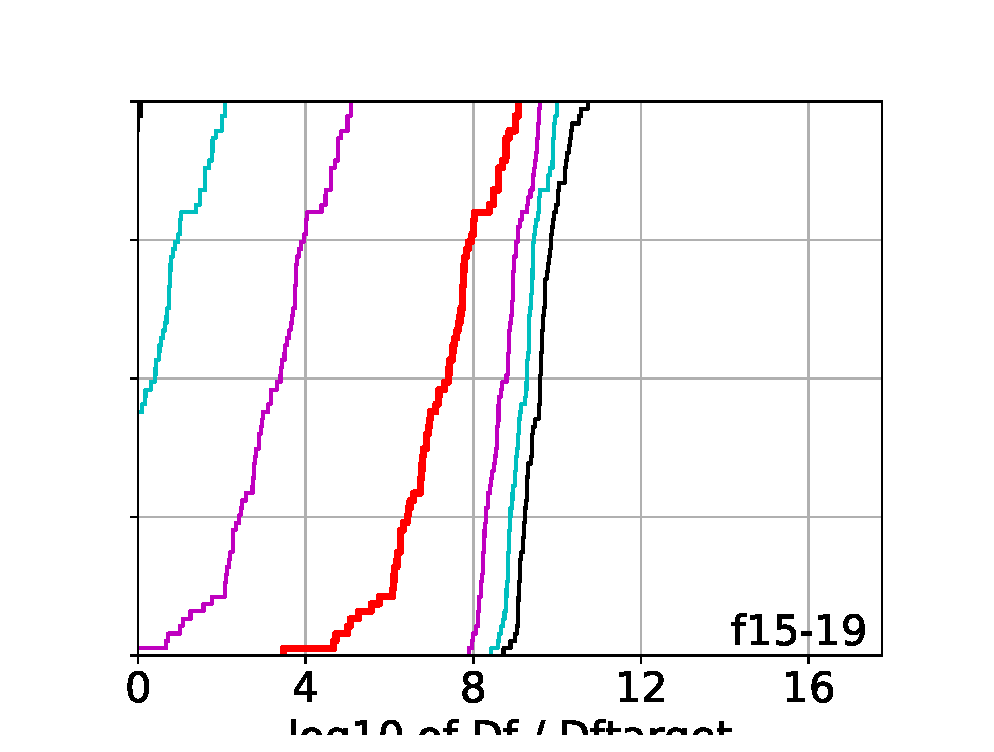
\includegraphics[width=0.2362\textwidth,trim=2.40cm 0 0 13mm, clip]{ppfvdistr_dim05multi} &
\includegraphics[width=0.268\textwidth,trim=0 0 0 13mm, clip]{pprldistr_dim20multi} &
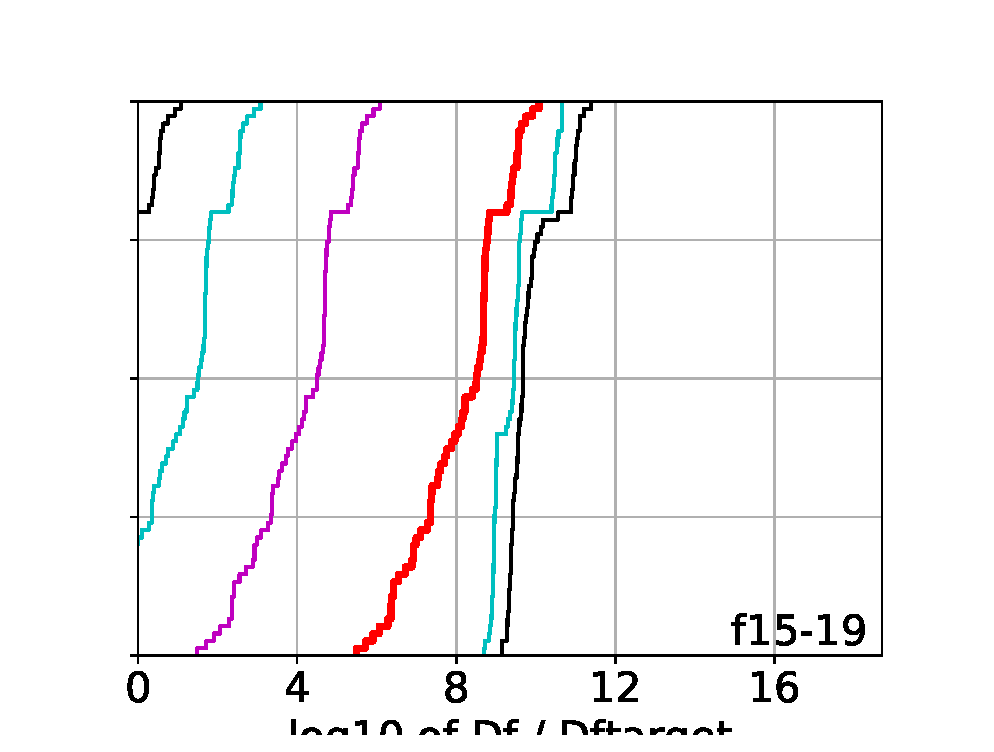
\includegraphics[width=0.2362\textwidth,trim=2.40cm 0 0 13mm, clip]{ppfvdistr_dim20multi} \\[-2ex]
\rot[1.0]{weak structure fcts}
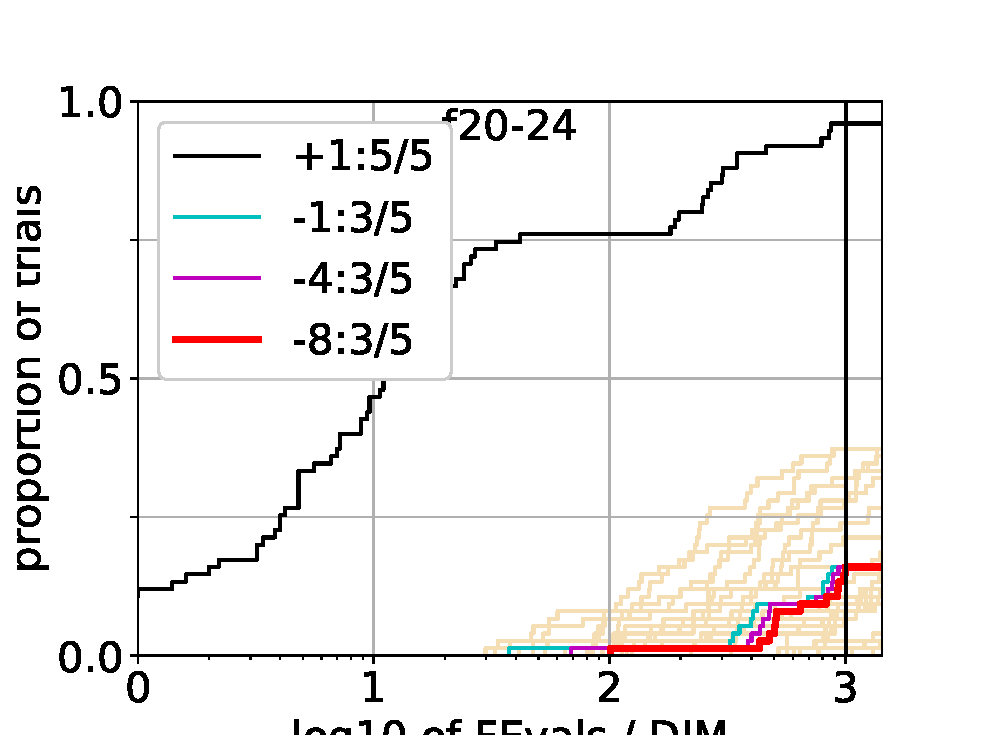
\includegraphics[width=0.268\textwidth,trim=0 0 0 13mm, clip]{pprldistr_dim05mult2} &
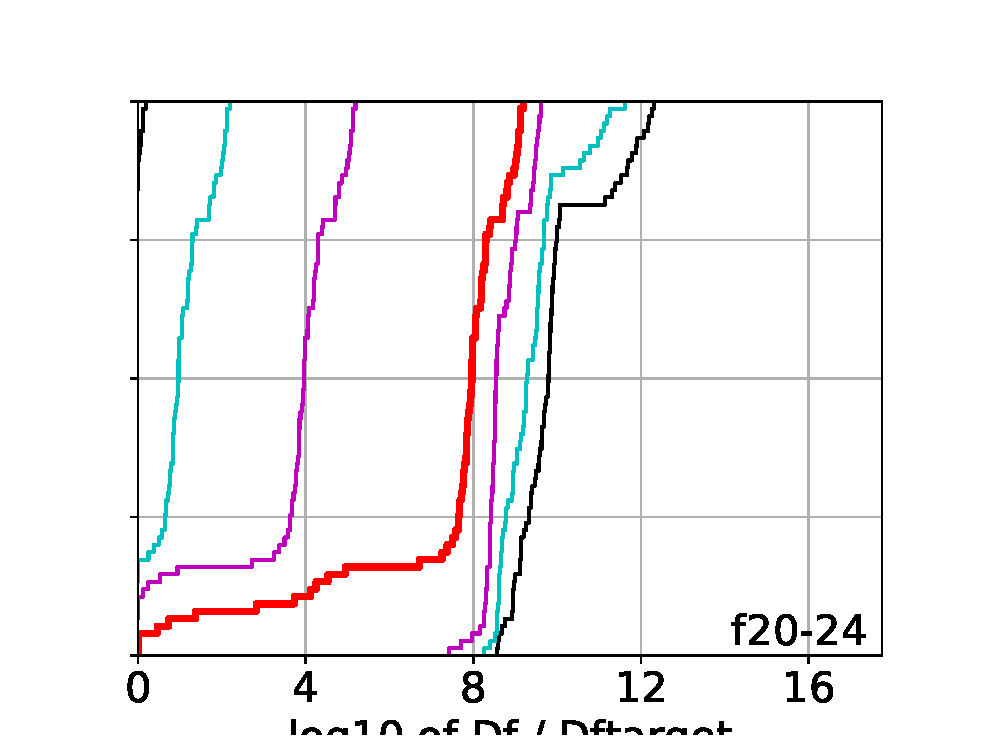
\includegraphics[width=0.2362\textwidth,trim=2.40cm 0 0 13mm, clip]{ppfvdistr_dim05mult2} &
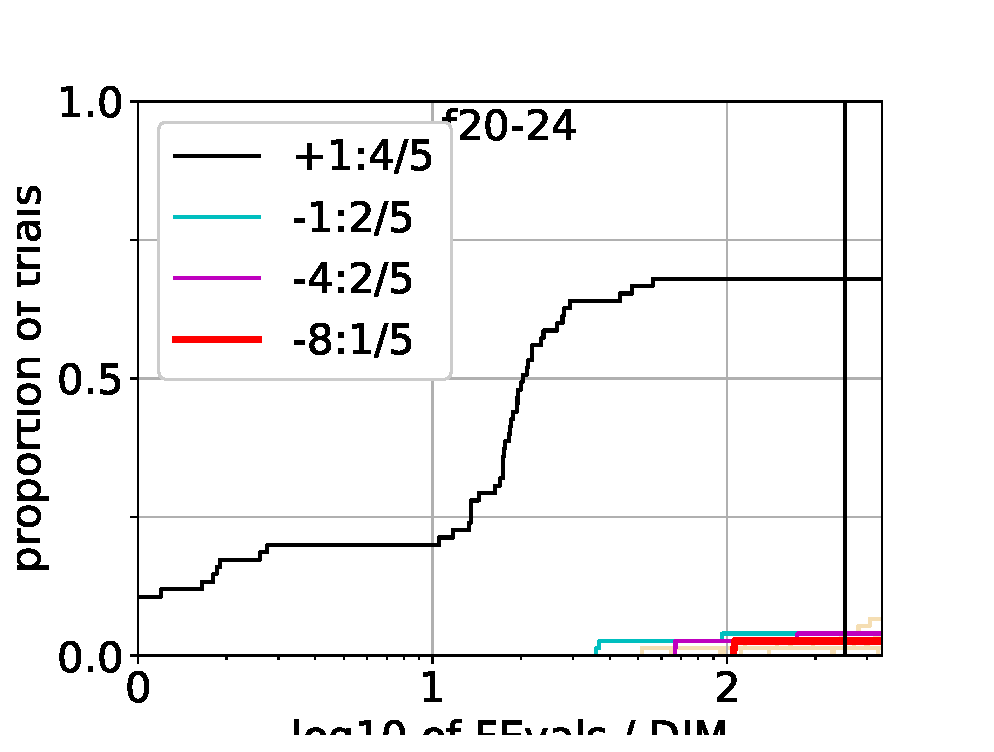
\includegraphics[width=0.268\textwidth,trim=0 0 0 13mm, clip]{pprldistr_dim20mult2} &
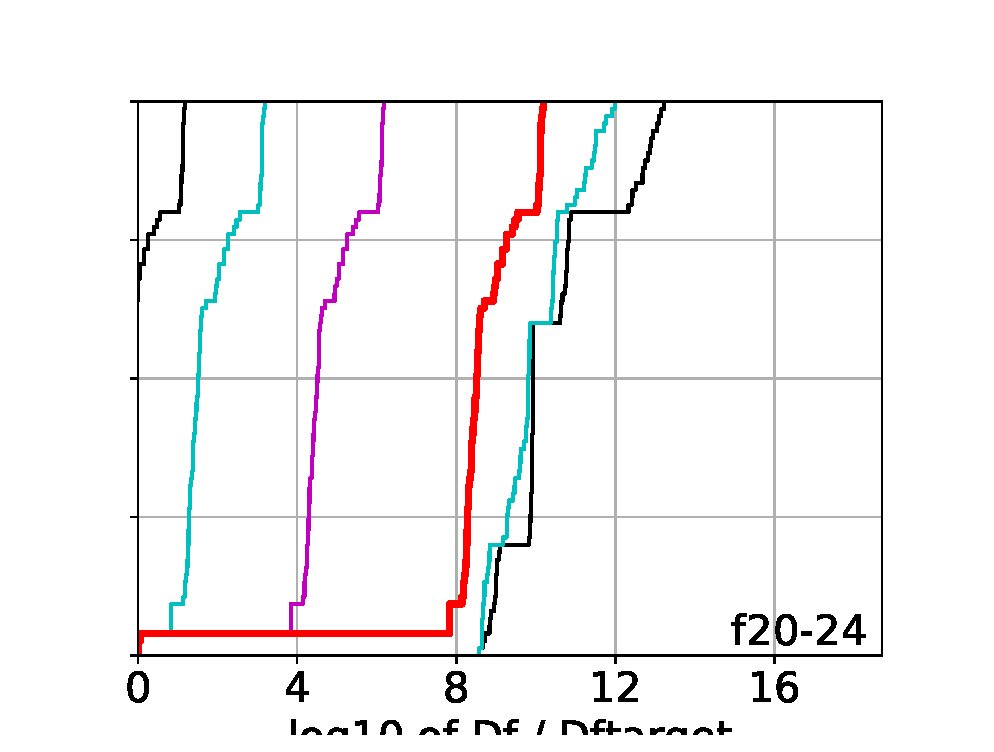
\includegraphics[width=0.2362\textwidth,trim=2.40cm 0 0 13mm, clip]{ppfvdistr_dim20mult2}
\vspace*{-0.5ex}
\end{tabular}
 \caption{\label{fig:RLDs}Empirical cumulative distribution functions (ECDFs), plotting the fraction of trials versus running time (left subplots) or versus \Df\ (right subplots).  The thick red line represents the best achieved results. Left subplots: ECDF of the running time (number of function evaluations), divided by
 search space dimension $D$, to fall below $\fopt+\Df$ with
 $\Df=10^{k}$, where $k$ is the first value in the legend. Right subplots: ECDF of the best achieved \Df\ divided by $10^k$ (upper left
 lines in continuation of the left subplot), and best achieved \Df\
 divided by $10^{-8}$ for running times of $D, 10\,D,
 100\,D\dots$ function evaluations (from right
 to left cycling black-cyan-magenta).
 %Top row: all functions; second row: separable
 %functions; third row: misc.\ moderate functions; fourth row:
 %ill-conditioned functions; fifth row: multi-modal functions with
 %adequate structure; last row: multi-modal functions with weak structure.
 The legends indicate the number of functions that were solved in at
 least one trial. FEvals denotes number of function evaluations,
 $D$ and \textsf{DIM} denote search space dimension, and \Df\ and \textsf{Df} denote the difference to the optimal function value.
 Light brown lines in the background show ECDFs for target value $10^{-8}$ of all algorithms benchmarked during BBOB-2009.}
\end{figure*}
%%%%%%%%%%%%%%%%%%%%%%%%%%%%%%%%%%%%%%%%%%%%%%%%%%%%%%%%%%%%%%%%%%%%%%%%%%%%%%%
%%%%%%%%%%%%%%%%%%%%%%%%%%%%%%%%%%%%%%%%%%%%%%%%%%%%%%%%%%%%%%%%%%%%%%%%%%%%%%%
%%%%%%%%%%%%%%%%%%%%%%%%%%%%%%%%%%%%%%%%%%%%%%%%%%%%%%%%%%%%%%%%%%%%%%%%%%%%%%%
\begin{figure}
\begin{tabular}{@{}l@{}@{}l@{}}
\multicolumn{1}{c}{5-D} & \multicolumn{1}{c}{20-D}\\
\rot{all functions}
\hspace*{-2mm}
\includegraphics[width=0.24\textwidth,trim=0 0 16mm 12mm, clip]{pplogloss_dim05noiselessall} &
\includegraphics[width=0.24\textwidth,trim=7mm 0 9mm 12mm, clip]{pplogloss_dim20noiselessall}\\[-2ex]
\rot{separable fcts}
\hspace*{-2mm}
\includegraphics[width=0.24\textwidth,trim=0 0 16mm 12mm, clip]{pplogloss_dim05separ} &
\includegraphics[width=0.24\textwidth,trim=7mm 0 9mm 12mm, clip]{pplogloss_dim20separ}\\[-2ex]
\rot[2]{moderate fcts}
\hspace*{-2mm}
\includegraphics[width=0.24\textwidth,trim=0 0 16mm 12mm, clip]{pplogloss_dim05lcond} &
\includegraphics[width=0.24\textwidth,trim=7mm 0 9mm 12mm, clip]{pplogloss_dim20lcond}\\[-2ex]
\rot[1.3]{ill-conditioned fcts}
\hspace*{-2mm}
\includegraphics[width=0.24\textwidth,trim=0 0 16mm 12mm, clip]{pplogloss_dim05hcond} &
\includegraphics[width=0.24\textwidth,trim=7mm 0 9mm 12mm, clip]{pplogloss_dim20hcond}\\[-2ex]
\rot[1.6]{multi-modal fcts}
\hspace*{-2mm}
\includegraphics[width=0.24\textwidth,trim=0 0 16mm 12mm, clip]{pplogloss_dim05multi} &
\includegraphics[width=0.24\textwidth,trim=7mm 0 9mm 12mm, clip]{pplogloss_dim20multi}\\[-2ex]
\rot[1.0]{weak structure fcts}
\hspace*{-2mm}
\includegraphics[width=0.24\textwidth,trim=0 0 16mm 12mm, clip]{pplogloss_dim05mult2} &
\includegraphics[width=0.24\textwidth,trim=7mm 0 9mm 12mm, clip]{pplogloss_dim20mult2}
\vspace*{-0.5ex}
\end{tabular}
 \caption{\label{fig:ERTlogloss}
\ERT\ loss ratio versus given budget $\FEvals$. 
%
The target value \ftarget\ for \ERT\ (see Figure~\ref{fig:ERTgraphs}) is the smallest (best) recorded 
function value such that $\ERT(\ftarget)\le\FEvals$ for the presented algorithm. 
%
Shown is \FEvals\ divided by the respective best $\ERT(\ftarget)$ from BBOB-2009 
%
for functions $f_1$--$f_{24}$ in 5-D and 20-D. 
%
Each \ERT\ is multiplied by $\exp(\CrE)$ correcting for the parameter crafting effort. 
Line: geometric mean. Box-Whisker error bar:
25-75\%-ile with median (box), 10-90\%-ile
(caps), and minimum and maximum \ERT\ loss ratio (points). The vertical line
gives the maximal number of function evaluations in this function subset.
}
\end{figure}

\begin{table}
\caption{\label{tab:ERTloss}\ERT\ loss ratio (see Figure~\ref{fig:ERTlogloss})
compared to the respective best result from BBOB-2009 for budgets given in the first
column. The last row $\text{RL}_{\text{US}}/\text{D}$ gives the number of function evaluations in 
unsuccessful runs divided by dimension. Shown are the smallest, 10\%-ile, 25\%-ile, 
50\%-ile, 75\%-ile and 90\%-ile value (smaller values are better).
}
\centering
\input{\bbobdatapath pploglosstable_dim05noiselessall}
\input{\bbobdatapath pploglosstable_dim20noiselessall}
\end{table}
%%%%%%%%%%%%%%%%%%%%%%%%%%%%%%%%%%%%%%%%%%%%%%%%%%%%%%%%%%%%%%%%%%%%%%%%%%%%%%%



%
% The following two commands are all you need in the
% initial runs of your .tex file to
% produce the bibliography for the citations in your paper.
\bibliographystyle{abbrv}
\bibliography{bbob}  % bbob.bib is the name of the Bibliography in this case
% You must have a proper ".bib" file
%  and remember to run:
% latex bibtex latex latex
% to resolve all references
% to create the ~.bbl file.  Insert that ~.bbl file into
% the .tex source file and comment out
% the command \texttt{{\char'134}thebibliography}.
%
% ACM needs 'a single self-contained file'!
%

\clearpage % otherwise the last figure might be missing
\end{document}
